\chapter{Evaluierung}
\label{evaluation}
%Die Beurteilung ist einer der wichtigsten Abschnitte der Arbeit
%- Sie enthält die Quintessenz des gesamten Projektes
%Viele lesen nur die Einführung und die Beurteilung an
%- Hier muss also alles Wichtige drin stehen!
%Hier beweisen Sie dass Sie …
%- die Aufgabe und deren Bedeutung verstanden haben
%- die Ergebnisse richtig zu interpretieren vermögen
%- wissen, worauf es bei diese Arbeit ankam


\section{Erfolgskriterien}
\label{sec:Erfolgskriterien}
Um die Fragestellung zu beantworten wird ein Probandentest mit Teilnehmern, die bereits Erfahrung mit Pen-\&-Paper-Rollenspiel gemacht haben, durchgeführt. Folgende Kriterien dienen am Ende des Projektes zur
Auswertung der Frage:

\begin{enumerate}
	\item Mindestens 66\% der Testspieler fühlen sich in ihrem Handlungsfreiraum nicht eingeschränkt. Im Probandentest soll ermittelt werden, ob Spieler sich subjektiv in ihrem Handlungsfreiraum eingeschränkt fühlen, also ob sie Aktionen ausführen möchten, auf die der Spielleiter nicht reagieren kann.
	\item Höchstens 33\% der Testspieler (inkl. Spielleiter) empfanden die Wartezeiten bei der Umsetzung ihrer Ideen durch den Spielleiter als zu lang. Im Probandentest soll ermittelt werden, ob der Spielleiter auf jede Situation in angemessener Zeit reagieren kann. Dies bedeutet, dass nur wenige Spieler in einer anschließenden Befragung angeben, durch lange Wartezeiten gestört worden zu sein.
	\item Der Spielleiter begreift die Standardfunktionen intuitiv und arbeitet eine Menge von Aktionen in vertretbarer Zeit ab. Der Spielleiter soll in der Lage sein, alle Funktionen, die das Spiel bietet (Objekte erstellen, platzieren, modifizieren, auf Spieleraktionen reagieren etc.), schnell zu begreifen und zu verwenden. Hierfür wird ein Satz von Aufgaben festgelegt, der diese Funktionen beinhaltet. Die Aufgaben müssen innerhalb festgelegter Zeiträume abgeschlossen werden. Die jeweilige Dauer kann der Aufgabenstellung im \hyperlink{AppendixSpielleiter.1}{Testszenario} entnommen werden.
\end{enumerate}

Dieser Probandentest wird über die zwei, im \hyperlink{AppendixFragebogenA.1}{Anhang referenzierten}, Formulare durchgeführt. Das erste Dokument ist ein Fragebogen und wird dabei von allen Teilnehmern ausgefüllt um ein Meinungsbild über verschiedenen Aspekte der Erfolgskriterien zu erhalten. Das zweite Dokument wird speziell von Spielleitern bearbeitet. Es enthält einige Aufgaben die häufiger in der Vorbereitung, bzw. Spielphase einer PnP Runde auftreten. Durch das Messen der benötigten Zeit soll ein Messwert generiert werden, der auf die Arbeitsgeschwindigkeit von Spielleitern schließen lässt.
  



\section{Testaufbau}
\label{sec:Testaufbau}
%\begin{itemize}
%	\item Anzahl der Testspiele
%	\item Anzahl Spieler
%	\item Anzahl unterschiedlicher Spieler / Spielleiter
%	\item Genaue Aufgabenstellung der Tests (Appendix: genau der Fragebogen, den wir rausgeben)
%\end{itemize}
Die Datenerhebung dieser Evaluierung wurde über einen Fragebogen durchgeführt, welcher während eines Probandentest von den Teilnehmern ausgefüllt wurde. Der Fragebogen enthält zehn Fragen, die dazu dienen die Rollenspielerfahrung der Testperson, sowohl digital als auch PnP, zu bestimmen (Frage 1 -3) und ein Qualitätslevel des Prototypen zu evaluieren (Frage 4-10). Die Fragen stellen in allen Fällen Aussagen dar, welche numerisch von 1 bis 4 vom Tester bewertet werden. Folgende Werte wurden dafür festgesetzt:

\begin{enumerate}
	\item Der Tester stimmt der Aussage gar nicht zu
	\item Der Tester stimmt der Aussage eher nicht zu
	\item Der Tester stimmt der Aussage eher zu
	\item Der Tester stimmt der Aussage voll und ganz zu
\end{enumerate}

Die Entscheidung eine Likert Skala\footnote{http://de.wikipedia.org/wiki/Likert-Skala, 18.03.14} mit nur 4 Punkten zu verwenden wurde getroffen, um die Tester zu einer eindeutigen Entscheidung für, oder gegen die Aussage zu zwingen. \cite{Garland1991} hebt hervor, dass bei dem Vorhandensein einer neutralen Option, diese oftmals im Gegensatz zu einer schlechteren Einschätzung zu wählen. In unserem Fall wurden die Tester an die Materie herangeführt und besaßen die nötigen Kenntnisse um die gestellten Aussagen zu bewerten. Die 4 Punkteskala sollte daher eine genauere Entscheidung provozieren ob die betrachteten Feature tatsächlich für die Umsetzung geeignet waren oder nicht.
Die Qualitätsfragen zahlen dabei auf die verschiedenen Erfolgskriterien ein. Mit der genannten Skala bedeutet dies im Detail, dass die Werte 3 und 4 ein erfülltes Erfolgskriterium bedeuten, während 1 und 2 das Erfolgskriterium nicht erfüllen. \newline
Insgesamt wurde die Auswertungen in \todo{Anzahl Testrunden} durchgeführt, wobei \todo{Anzahl Spieler} und \todo{Anzahl Spielleiter} die Fragen ausgefüllt haben. Alle befragten Spieler hatten bereits umfassende Erfahrungen mit PnP Rollenspielen als Spieler und über zwei Drittel haben ebenfalls schon als Spielleiter agiert. Auch bei digitalen Rollenspiele gaben alle Probanden umfassende Kenntnisse an. 



\section{Auswertung}
\label{sec:Auswertung}

In diesem Abschnitt werden die erhobenen Daten in Bezug gesetzt und anhand dieser die Erfolgskriterien evaluiert.


\subsection{Handlungsfreiheit}
\label{sec:Handlungsfreiheit}
Der wohl elementarste Faktor des Prototypen war die Handlungsfreiheit von Spielern und Spielleiter. Dieser Aspekt wird durch die Fragen 4 und 5 auf \emph{Fragebogen A} evaluiert. Zum einen wurde beleuchtet, ob Spieler und Spielleiter sich in der Lage fühlten ihre eigenen Ideen im Spielfluss umzusetzen und damit ihre Kreativen Lösungsstrategien einzubringen, zum anderen wurde ausgeschlossen, dass das Spielsystem den Handlungsfreiraum der Tester einschränkt.\newline
\ref{fig:questions_4_5} zeigt die Box-Plot Auswertung dieser Fragen. Der Grafik ist zu entnehmen, dass die Tester während der Probespiels ihre Ideen vollständig umsetzen \todo{(Mittelwert: 4)} konnten und sich nahezu nicht in ihrer Handlungsfreiheit eingeschränkt fühlen \todo{(Mittelwert: 3,57)}. Insgesamt ergibt sich daher, bei einer Gleichgewichtung beider Fragen ein Durchschnittswert von \todo{3,79}. Zur erfolgreichen Erfüllung des Erfolgskriterium müssen mindestens 66\% der Tester sich nicht in der Handlungsfreiheit eingeschränkt fühlen, mit der in \ref{sec:Testaufbau} vorgestellten Skala bedeutet dies, dass 66\% der Tester die Aussagen mit 3 oder 4 bewerten.\newline
Die Auswertung zeigt, dass alle Tester die Fragen mit 3 oder besser bewertet haben. Damit ist gezeigt, dass die Umsetzung eigener Ideen durch den Prototypen möglich ist und Spieler einen Freiraum erfahren, der sonst hauptsächlich aus PnP-Rollenspielen bekannt ist.

\begin{figure}
	\centering
		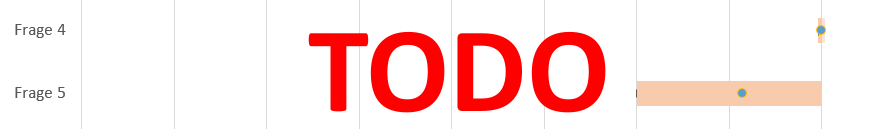
\includegraphics[width=1.00\textwidth]{media/2questions_temp.png}
	\caption{Auswertung von Frage 4 und 5}
	\label{fig:questions_4_5}
\end{figure}
	

\subsection{Umsetzungszeit während des Spiels}
\label{sec:Umsetzungszeit}
Um eine Entwicklung der Geschichte und ein immersives Spielgefühl zu ermöglichen darf der Prototyp nicht unverhältnismäßig langsamer sein als die normale Arbeitsweise eines Spielleiters. Benötigt der Spielleiter sehr lange um Aktionen umzusetzen, oder brauchen die Spieler viel Zeit um Werte einzugeben und Aktionen zu formulieren, so wird der Spielfluss gebrochen. Die Fragen 6 und 7 evaluieren daher das zweite Erfolgskriterium, welches fordert, dass die Umsetzungszeit der eigenen Ideen, sowie die Reaktionszeit des Spielleiters in einem annehmbaren Rahmen liegen.
\todo{endgültige auswertung der grafik}

Der Prototyp erfüllt damit auch das zweite Erfolgskriterium und erlaubt es Spielern und Spielleitern in einem angemessen Tempo zu agieren und das erdachte Abenteuer zu erfahren.

\begin{figure}
	\centering
		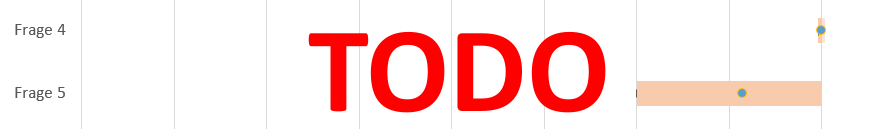
\includegraphics[width=1.00\textwidth]{media/2questions_temp.png}
	\caption{Auswertung von Frage 6 und 7}
	\label{fig:questions_6_7}
\end{figure}


\subsection{Umsetzungszeit und Bedienung durch den Spielleiter}
\label{sec:UmsetzungszeitUndBedienungDurchDenSpielleiter}
Für das dritte Erfolgskriterium würde in \emph{Fragebogen B} ein Set von Aufgaben definiert und mit Zeiten versehen. Diese Aufgaben stellen eine Querschnitt der regulären Tätigkeiten eines Spielleiters vor und während einer Spielrunde dar. Im Probandentest wurden die Tester mit Spielleiter-Erfahrung aufgefordert diese Aufgaben abzuarbeiten während die Zeit festgehalten wurde. Der Fragebogen enthält sowohl zeitlich bestimmte Aufgaben, welche das Vorbereiten und Erstellen eines Abenteuers beinhalten, als auch zeitlich unbestimmte Aufgaben welche das eigentliche Rollenspiel darstellen. Die Entscheidung Zweitere ohne zeitlichen Rahmen vorzugeben wurde getroffen, um spontanes Rollenspiel (Wie zum Beispiel Armdrücken in der Taverne) zu ermöglichen. Der flüssige Ablauf dieser zweiten Aufgaben spiegelt sich in Frage 6 und 7 wieder. Im Verlaufe dieses Tests erstellt der SL eine kleine Verlies Karte mit drei Räumen. Raum 1 enthält einen Interaktions-Gegenstand, Raum 2 eine kleine Gruppe Gegner und Raum 3 eine Schatztruhe.\newline
Beim Bespielen beginnt die Gruppe in einer vordefinierten Taverne und wird vom SL durch Rollenspiel in das Verlies geführt wo sie die drei Räume meistern muss. Dieser Test orientiert sich dabei an dem im \ref{sec:Spielfluss} verwendeten Szenario und soll eine breite Übersicht über die Funktionen des Prototypen bieten.\newline
\ref{tab:FragebogenB} zeigt eine Aufschlüsselung der verschiedenen, zeitlich gewichteten, Aufgaben. Dargestellt werden die einzelnen Tätigkeiten, die veranschlagten Zeiten und die im Durchschnitt benötigten Zeiten, diese wurden von dem Testleiter während der Ausführung gemessen. Aus der Tabelle lässt sich entnehmen, dass der SL bei allen Aufgaben schneller arbeiten konnte als veranschlagt wurde. Daraus, in Kombination mit dem zweiten Erfolgskriterium, lässt sich auf eine intuitive Bedienung des Prototypen schließen. Spielleiter konnten ohne große Einarbeitung Funktionen begreifen und schnell eigenen Ideen und Konzepte über die vorgegebenen Arbeitsschritte umsetzen. 
\begin{table}

\begin{tabularx}{\textwidth}{|X|l|l|}
\hline
Aufgabe & Zeit geplant (min) & \O Zeit (min)\\
\hline
\hline
Erstellen einer neuen Karte & 2 & 0.88 \\
\hline
Anlegen von 3 Räumen & 5 & 2 \\
\hline
Erstellen eines Gegners & 3 & 2,8 \\
\hline
Erstellen eines Interaktionsgegenstands & 2 & 1,1 \\
\hline
Platzieren von Gegnern & 1 & 0 \\
\hline
Platzieren und Füllen der Schatztruhe & 2 & 1,5 \\

\hline
\end{tabularx}
\caption{Auswertung von Fragebogen B}
	\label{tab:FragebogenB}
\end{table}






